\section{行銷策略}

\subsection{目標消費族群}
\par 經由網路調查發現,在新北或北部郊外地區的偏鄉學校,普遍對於資訊教育較為不重視。主要問題包括硬體設備不齊全、專業師資不足,導致學校不重視資訊知識。考慮到現今升學制度偏向專業發展,位於偏鄉地區的學生能夠使用本身的專業知識,來前往更前端的大學或其他學校機構,增加升學的可能性。
\par 程式教學是我們團隊的強項,我們認為這是解決偏鄉學校資訊教育不足的商機。我們打算與教育機構合作,提供針對偏鄉高中職學校缺少的資訊教育能力的教學軟體即服務(SaaS),以相對負擔得起的價格來提供更好的教育資源,以平衡偏鄉地區的資源分配問題,這正是我們發現的商機所在。

\begin{table}[H]
  \centering
  \begin{tabular}{|c|c|c|}
    \hline
    \multicolumn{2}{|c|}{服務模式} & \\
    \hline
    \multirow{5}{*}{目標消費族群} & 身分 & 教師 \\
    \cline{2-3}
    ~ & 性別 & 不限 \\
    \cline{2-3}
    ~ & 收入 & 不限 \\
    \cline{2-3}
    ~ & 居住地區 & 目前限中文用語地區 \\
    \cline{2-3}
    ~ & 擁有共通興趣 &
    \begin{minipage}[c]{0.5\columnwidth}
      \vspace{0.5em}
      \begin{enumerate}[label=(\arabic*)]
        \setlength{\parindent}{1em}
        \item 資訊設備或師資不足的教學機構
        \item 學生對於資訊相關教育有興趣的教育場所
      \end{enumerate}
      \vspace{0.1em}
    \end{minipage} \\
    \hline
    \multirow{5}{*}{目標使用族群} & 身分 & 教育者 \\
    \cline{2-3}
    ~ & 性別 & 不限 \\
    \cline{2-3}
    ~ & 收入 & 不限 \\
    \cline{2-3}
    ~ & 居住地區 & 目前限中文用語地區 \\
    \cline{2-3}
    ~ & 擁有共通興趣 & 
      \begin{minipage}[c]{0.45\columnwidth}
        \vspace{0.5em}
        \begin{enumerate}[label=(\arabic*)]
          \setlength{\parindent}{2em}
          \item 想給予學生更多吸收資訊知識的導師
          \item 無法解決學校設備缺乏的困擾
        \end{enumerate}
        \vspace{0.1em}
      \end{minipage} \\
    \hline
  \end{tabular}
  \caption{商業服務模式表,資料來源:團隊自行設計}
\end{table}
\newpage
\subsection{行銷策略}

\begin{enumerate}[label=(\arabic*)]
  \item 過去的行銷成果
    \par 已於Instagram、Facebook、普羅官網(線上學習平台)共三個社群平台上,推廣科普文章、普羅課程資訊及資訊時事供社群大眾閱讀,增加品牌信心與知名度。
    \begin{figure}[H]
      \centering
      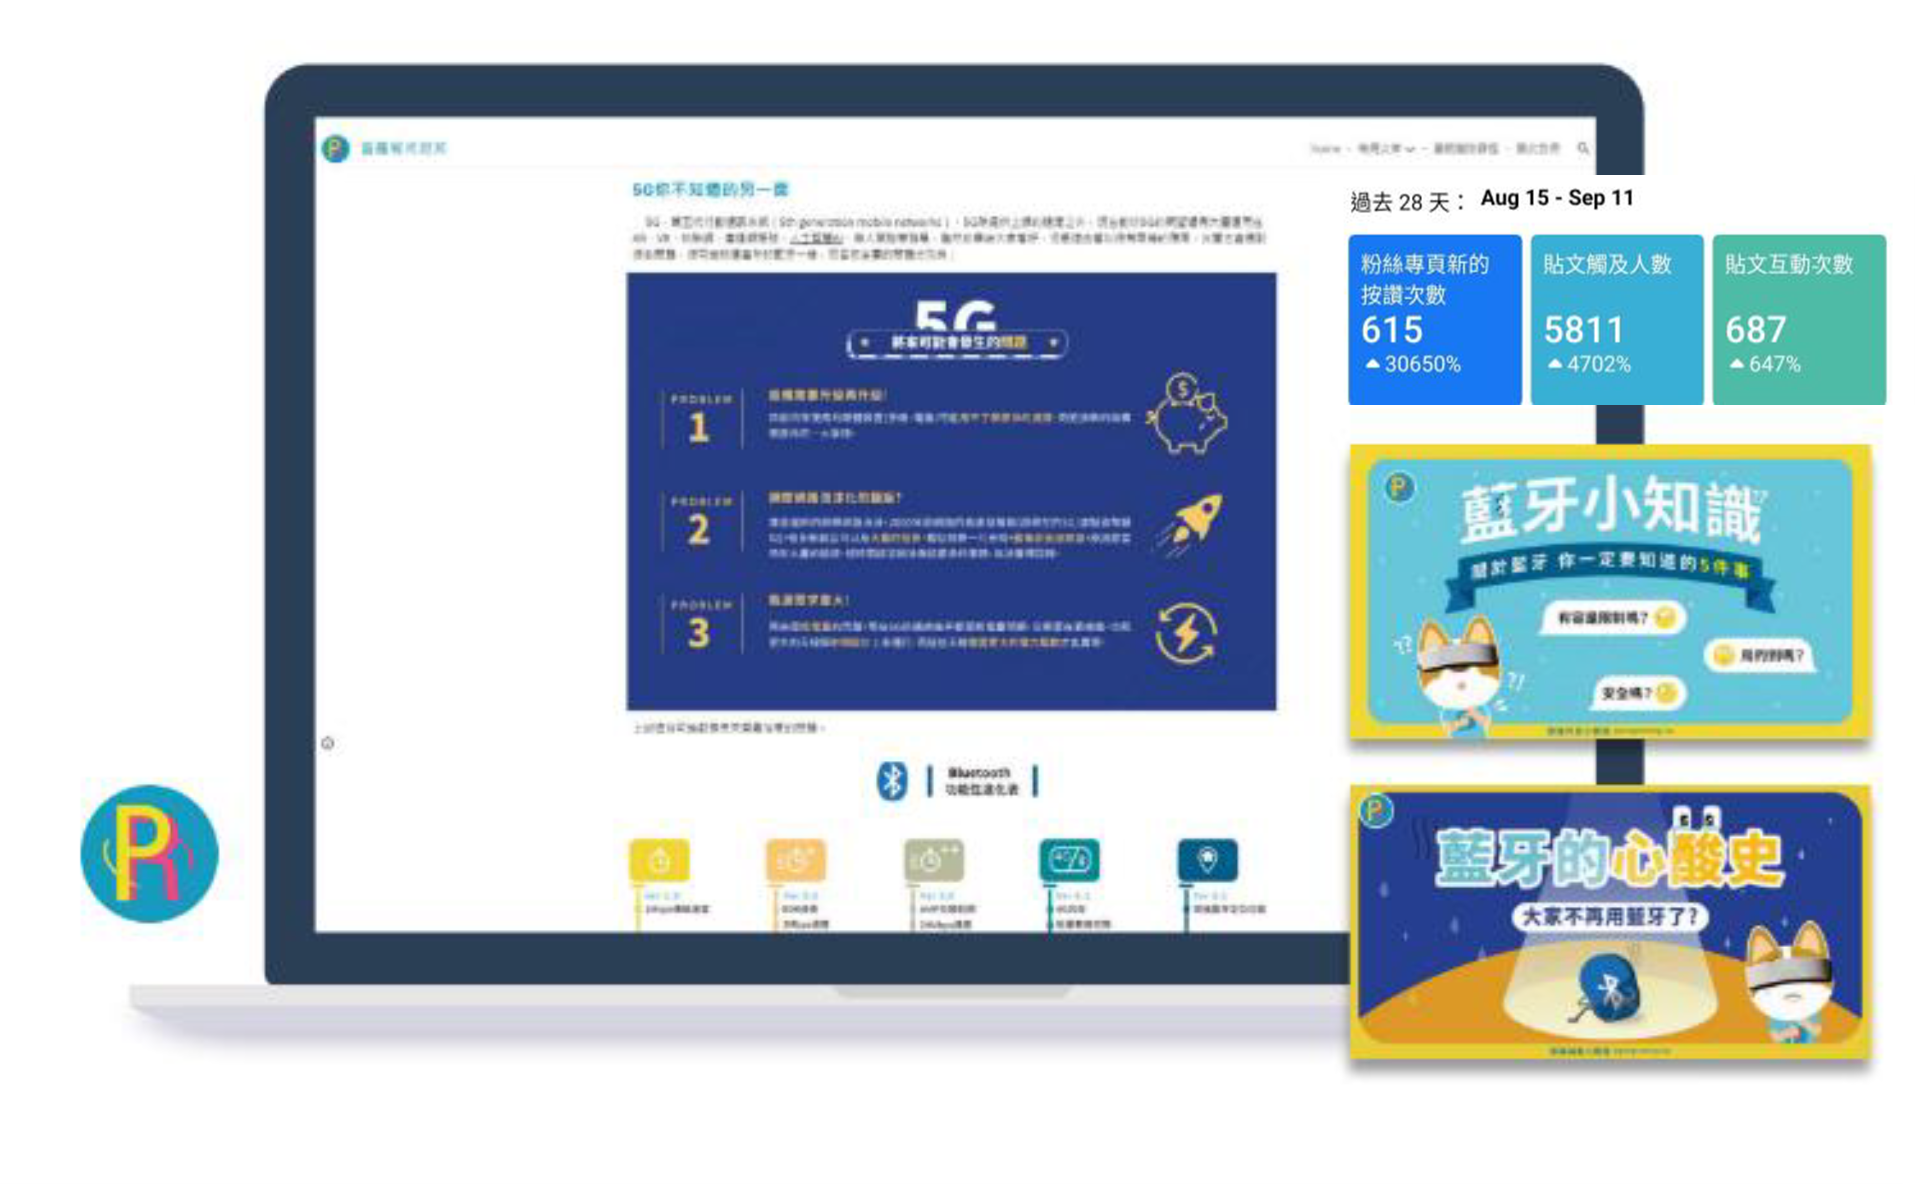
\includegraphics[width=0.6\textwidth]{./Strategies/img/article.png}
      \caption{科普文章,資料來源:團隊自行設計}
  	\end{figure}
  \item 目前的行銷規劃
  	\par 以熟識的老師作為第一批試用目標,地區為新北偏鄉學校。我們將積極收集老師的回饋,包括他們對工具的使用感受、意見和建議。我們會與這些老師建立密切的合作關係,並請他們分享他們的使用經驗,以便建立我們的口碑。
  	\par 在增加功能及知名度後,我們計劃透過線上和線下說明會的方式,向更多的新北偏鄉或北部郊區學校建立販售及獲取的橋樑。同時,我們也會利用老師們的口碑推薦,加強我們在目標客戶群體中的知名度,並吸引更多的潛在客戶。
  \item 未來的行銷規劃
  	\par 在完善功能與建立一定知名度後,我們計畫與個人教師合作,如:試用並分享心得、推薦給其他使用者並獲得優惠、擔任合作教師並錄製課程供宣傳以及與教育機構建立合作夥伴關係,提供定制化的解決方案和支持服務。透過與個人教師和教育機構的合作更好地了解客戶需求,持續改進產品功能,並擴大市場覆蓋範圍。我們也將持續投資於市場營銷和品牌宣傳,提升產品知名度和品牌價值,以吸引更多的客戶和合作夥伴加入我們的生態系統。
\end{enumerate}
